% =====================================================================
%  Estimating carbohydrate and fat oxidation from heart rate and
%  Garmin's energy estimate (paper, English version)
%  Translated on 21/11/2026 from oxidacio-energia-dispositiu.tex (points 1-77).
%  Compile: pdflatex model-fc-energia.en.tex (two passes)
% =====================================================================
\documentclass[10pt,a4paper]{article}

\usepackage[utf8]{inputenc}
\usepackage[T1]{fontenc}
\usepackage[english]{babel}
\usepackage{lmodern}
\usepackage{microtype}
\usepackage[a4paper,margin=2.4cm]{geometry}
\usepackage{amsmath,amssymb}
\usepackage{booktabs}
\usepackage{tabularx}
\usepackage{array}
\usepackage{caption}
\usepackage{float}
\usepackage{needspace}
\usepackage{enumitem}
\usepackage{tikz}
\usetikzlibrary{positioning,arrows.meta}
\usepackage{pgfplots}
\pgfplotsset{compat=1.17}
\usepackage[most]{tcolorbox}
\usepackage[numbers,sort&compress]{natbib}
\usepackage[hidelinks]{hyperref}

\captionsetup{font=small,labelfont=bf}
\renewcommand{\arraystretch}{1.25}
\newcolumntype{L}{>{\raggedright\arraybackslash}X}
\setlist{itemsep=2pt,topsep=4pt}

% Green box for the checks (the full title is passed as a parameter)
\newtcolorbox{requadre}[2][]{enhanced, colback=green!4, colframe=green!45!black,
  boxrule=0.6pt, arc=2pt, left=6pt, right=6pt, top=4pt, bottom=4pt,
  fonttitle=\bfseries\small, title={$\checkmark$\ #2}, #1}

% Blue box for the conclusions of a section
\newtcolorbox{conclusio}{enhanced, colback=blue!4, colframe=blue!50!black,
  boxrule=0.6pt, arc=2pt, left=6pt, right=6pt, top=4pt, bottom=4pt,
  fonttitle=\bfseries\small, title={Conclusion}}

% Project website (it will change: edit it only here)
\newcommand{\webprojecte}{\url{https://irazuzta.github.io/ChoFatMetabolic/}}

% --- Notation ---------------------------------------------------------
\newcommand{\sub}[1]{{\scriptscriptstyle\mathrm{#1}}}   % small subscripts
\newcommand{\CHO}{\sub{CHO}}
\newcommand{\FAT}{\sub{FAT}}
\newcommand{\tot}{\sub{total}}
\newcommand{\smax}{{\scriptscriptstyle\text{max}}}
\newcommand{\cho}{\ensuremath{\mathit{CHO}}}               % oxidation rate (g/min)
\newcommand{\fat}{\ensuremath{\mathit{FAT}}}
\newcommand{\VO}{\ensuremath{\mathit{VO}_2}}               % rate (L/min)
\newcommand{\VCO}{\ensuremath{\mathit{VCO}_2}}
\newcommand{\VOmax}{\ensuremath{\mathit{VO}_{2\smax}}}
\newcommand{\RER}{\ensuremath{\mathit{RER}}}
\newcommand{\RERi}{\ensuremath{\overline{\mathit{RER}}}}
\newcommand{\FC}{\ensuremath{\mathit{HR}}}
\newcommand{\FCmax}{\ensuremath{\mathit{HR}_{\smax}}}
\newcommand{\Ion}{\ensuremath{I_{\mathrm{onset}}}}
\newcommand{\kcal}{\ensuremath{\mathrm{kcal}}}

\title{\textbf{Estimating carbohydrate and fat oxidation\\
from heart rate and Garmin's energy estimate}}
\author{Jordi Irazuzta\\
\small\href{mailto:irazuzta@gmail.com}{\texttt{irazuzta@gmail.com}}\\[4pt]
\small CHO/FAT Metabolic Pro project --- \webprojecte}
\date{Draft --- November 2026}

\begin{document}
\maketitle

\begin{abstract}
\noindent
This work estimates the rate of carbohydrate (CHO) and fat (FAT) oxidation during
exercise. This information can be used, for example, to decide how much carbohydrate to
take in. Indirect calorimetry computes it with the equations of Jeukendrup and Wallis, but
it needs a gas analysis to measure oxygen uptake (\VO) and the respiratory exchange ratio
(\RER). Here we estimate it from a sports watch that measures heart rate (\FC) and gives an
estimate of the energy expended; specifically, Garmin devices. The method starts from one
condition: the energy of the computed grams must be exactly the energy given by Garmin.
The \RER\ is estimated from \FC. The \VO\ is obtained by dividing the energy by the energy
released per litre of oxygen. This value is computed with the same equations of Jeukendrup
and Wallis and with the energy per gram of carbohydrate (4.1~kcal) and fat (9.3~kcal),
values that are supported by classical calorimetry. In this way, the condition holds
exactly. We also study the error as a function of the \RER, how to go from rates to
totals, the sources of error and how to apply the method in real time.
\end{abstract}

\noindent\textbf{Keywords:} substrate oxidation; indirect calorimetry; oxygen uptake;
respiratory exchange ratio; energy expenditure; wearable devices.

% =====================================================================
\section{Aim}\label{sec:objectiu}
% =====================================================================

We want to estimate, at each instant $t$ of the activity, the \textbf{oxidation rate} of
carbohydrate and fat:
\[
  \cho(t),\ \fat(t)\qquad[\mathrm{g/min}],
\]
and, from these rates, the \textbf{cumulative total} for the whole activity, from 0 to the
total duration $T$:
\begin{equation}
  \cho_{\tot}(T)=\int_0^T\cho(t)\,dt,\qquad
  \fat_{\tot}(T)=\int_0^T\fat(t)\,dt .
  \label{eq:totals}
\end{equation}
The integral is the cumulative total: everything oxidised from the start up to $T$.
Section~\ref{sec:total} explains how it is computed with Garmin data. If desired, this
information can help decide how much carbohydrate to take in during exercise
\citep{jeukendrup2014}.

\paragraph{The approach.} Indirect calorimetry computes these rates from respiratory gases
(section~\ref{sec:jw}), but it needs a gas analyser. Here we estimate them with Garmin
devices (watches and Edge bike computers), which measure \FC\ and estimate the energy
expended. The steps are:
\begin{enumerate}[leftmargin=*,itemsep=0pt]
  \item From Garmin we obtain the energy expended, $E(t)$ (section~\ref{sec:energia}).
  \item The \RER\ is estimated from \FC\ (section~\ref{sec:rer}).
  \item From the \RER\ and $E(t)$ we can estimate \VO\ (section~\ref{sec:vo2}).
  \item With \VO\ and the \RER, the equations of Jeukendrup and Wallis give $\cho(t)$ and
        $\fat(t)$ (section~\ref{sec:jw}).
\end{enumerate}

\paragraph{Why this approach.} Another option is to estimate oxygen uptake from \FC, with a
fixed relationship between the two \citep{swain1997,chofatfc2026}. But then the energy that
comes out of the computed grams does not match the energy shown by Garmin: it tends to be
higher. Garmin uses more information: besides \FC, the user profile and each person's
relationship between \FC\ and oxygen uptake \citep{firstbeat2007}.

That is why this work starts from a \textbf{condition}: the energy of the computed grams
must be exactly the energy given by Garmin. Half-jokingly, we call it the ``Garmin energy
conservation principle'', by analogy with the law of physics: here the energy is set not
by nature, but by Garmin. The method does not recompute the energy; it only splits it
between the two fuels. This condition is what determines everything
(section~\ref{sec:vo2}). The rest of the approach and the notation follow the model that
estimates oxygen uptake from \FC\ \citep{chofatfc2026}.

\paragraph{Outline.} Section~\ref{sec:conceptes} introduces the necessary concepts. Then we
answer, in order, two questions: \textbf{how} $\cho(t)$ and $\fat(t)$ \textbf{are computed}
(sections~\ref{sec:jw}--\ref{sec:sensibilitat}) and \textbf{how the totals are computed}
(section~\ref{sec:total}). At the end there is an example, the sources of error and how to
apply the method in real time.

% =====================================================================
\section{Background}\label{sec:conceptes}
% =====================================================================

\subsection{Oxygen uptake (\texorpdfstring{$\mathit{VO}_2$}{VO2}) and CO\texorpdfstring{$_2$}{2}
output (\texorpdfstring{$\mathit{VCO}_2$}{VCO2})}\label{sec:gasos}
$\VO(t)$ is the volume of oxygen the body takes up per unit of time. It is measured in
L/min (absolute value) or in mL$\cdot$kg$^{-1}\cdot$min$^{-1}$ (relative to body mass, to
compare people). In the same way, $\VCO(t)$ is the volume of carbon dioxide produced per
unit of time. Both are the basis of \emph{indirect calorimetry}: oxidising fat or
carbohydrate uses O$_2$ and produces CO$_2$ in different proportions, so by measuring $\VO$
and $\VCO$ we can tell which fuel is being burned without measuring it directly.

\subsection{Maximal oxygen uptake (\texorpdfstring{$\mathit{VO}_{2\max}$}{VO2max})}
$\VOmax$ is the highest value of $\VO$ a person can reach. Here it is only used to express
intensities (for example, ``at 63\,\% of $\VOmax$'') and to detect impossible values of
$\VO(t)$.

\subsection{Respiratory exchange ratio (\texorpdfstring{$\mathit{RER}$}{RER})}
\begin{equation}
  \RER(t)=\frac{\VCO(t)}{\VO(t)} .
  \label{eq:rer-def}
\end{equation}
It is a single number that shows the fuel mix. Oxidising glucose produces as much CO$_2$ as
the O$_2$ it uses ($\RER=1$), whereas oxidising fat produces less ($\RER\approx0.70$).
During submaximal exercise it takes values between these two extremes \citep{peronnet1991}.
It is the key variable for the split between carbohydrate and fat.

\subsection{Energy estimated by Garmin devices}\label{sec:energia}
Garmin devices compute the energy of the activity with a method by Firstbeat, a Finnish
company specialised in physiological analysis based on heart rate; its consumer division
(Firstbeat Analytics) has been part of Garmin since 2020. The method uses \FC\ and the user
profile, and it takes into account each person's relationship between \FC\ and oxygen
uptake \citep{firstbeat2007}. We call $E(t)$ the \emph{rate} of energy expenditure, in
kcal/min, and $E_{\tot}(t)$ the \emph{cumulative} energy since the start, in kcal:
\begin{equation}
  E_{\tot}(t)=\int_0^t E(s)\,ds .
  \label{eq:etotal}
\end{equation}
Garmin gives $E_{\tot}(t)$; the rate $E(t)$ is obtained from the increments of this counter
(section~\ref{sec:total}). It is the \emph{total} energy: it also includes the resting
metabolism during that time (Garmin Connect splits it into resting and active calories).
This is the energy we need, because the calorimetry equations count all the oxidation from
all the oxygen used. It is an estimate, not a measurement: studies on wearable devices find
larger errors in it than in the measurement of \FC\ \citep{shcherbina2017,fuller2020}.

\needspace{10cm}
\subsection{Notation}
Table~\ref{tab:notacio} lists the symbols used in this work.

\begin{table}[H]
\centering
\caption{Notation.}
\label{tab:notacio}
\small
\begin{tabularx}{\textwidth}{@{}l L l@{}}
\toprule
Symbol & Meaning & Units \\
\midrule
$\cho(t)$, $\fat(t)$ & Carbohydrate and fat oxidation rate (the result) & g/min \\
$\cho_{\tot}(T)$, $\fat_{\tot}(T)$ & Total oxidised from the start up to $T$ & g \\
$\VO(t)$, $\VCO(t)$ & O$_2$ uptake and CO$_2$ output & L/min \\
$\RER(t)$ & Respiratory exchange ratio, $\VCO/\VO$ & --- \\
$E_{\tot}(t)$ & Cumulative energy since the start (given by Garmin) & kcal \\
$E(t)$ & Rate of energy expenditure (obtained from $E_{\tot}$) & kcal/min \\
$g_{\CHO}(\RER)$, $g_{\FAT}(\RER)$ & Grams of substrate oxidised per litre of O$_2$ & g/L \\
$e_{\CHO}$, $e_{\FAT}$ & Energy per gram of oxidised substrate; constants: 4.1 and 9.3 & kcal/g \\
$k(\RER)$ & Energy released per litre of O$_2$ & kcal/L \\
$\FC(t)$, $LT_1$, $LT_2$, $\FCmax$, $\Ion$ & Heart rate and \RER\ reference points & bpm \\
\bottomrule
\end{tabularx}
\end{table}

% =====================================================================
\section{The starting point: the equations of Jeukendrup and Wallis}\label{sec:jw}
% =====================================================================

The relationship between the oxygen used, the CO$_2$ produced and the grams of substrate
oxidised is known from the classical indirect calorimetry equations of
\citet{frayn1983}. They are ``non-protein'' equations: they assume that all the energy comes
from carbohydrate and fat, and they ignore protein oxidation, which provides little energy
during exercise. This work uses the exercise version by \citet{jeukendrup2005}:
\begin{align}
  \cho(t) &= 4.210\cdot\VCO(t)-2.962\cdot\VO(t), \label{eq:jw-cho}\\
  \fat(t) &= 1.695\cdot\VO(t)-1.701\cdot\VCO(t), \label{eq:jw-fat}
\end{align}
with gases in L/min and the result in g/min.

\paragraph{What is needed to use them?} The two variables of section~\ref{sec:gasos}:
$\VO(t)$ and $\VCO(t)$. Neither can be measured without a gas analyser, so they have to be
estimated.

\subsection{Rewriting the equations with the RER}\label{sec:jw-rer}
Instead of estimating $\VO$ and $\VCO$ separately, it is more practical to estimate $\VO$
and the \RER~\eqref{eq:rer-def}. Substituting $\VCO(t)=\RER(t)\cdot\VO(t)$:
\begin{align}
  \cho(t) &= \VO(t)\cdot\bigl(4.210\cdot\RER(t)-2.962\bigr), \label{eq:jw-cho-rer}\\
  \fat(t) &= \VO(t)\cdot\bigl(1.695-1.701\cdot\RER(t)\bigr). \label{eq:jw-fat-rer}
\end{align}

\paragraph{The extremes.} Outside the range 0.704--0.9965 one of the two brackets becomes
negative; that is why it is set to zero ($\cho=0$ below, $\fat=0$ above).

\needspace{12cm}
\paragraph{Two estimates are now needed:} $\RER(t)$ (section~\ref{sec:rer}) and $\VO(t)$
(section~\ref{sec:vo2}). The \RER\ comes first, because it is needed to estimate $\VO$.
Figure~\ref{fig:esquema} summarises the path.

\begin{figure}[H]
\centering
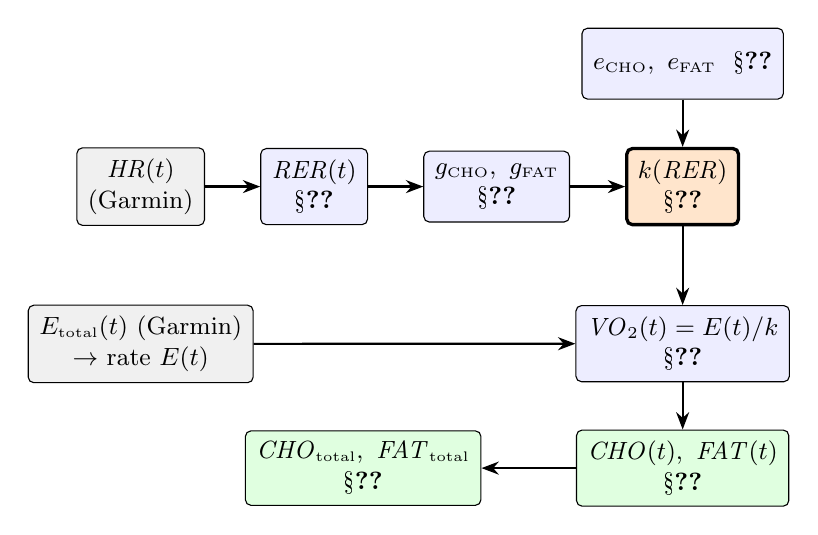
\begin{tikzpicture}[
  node distance=6mm and 7mm,
  caixa/.style={draw, rounded corners=2pt, align=center, font=\small, minimum height=9mm, inner sep=4pt},
  dada/.style={caixa, fill=gray!12},
  pas/.style={caixa, fill=blue!7},
  clau/.style={caixa, fill=orange!20, very thick},
  res/.style={caixa, fill=green!12},
  fl/.style={-{Stealth[length=2.2mm]}, thick}]
\node[dada] (fc) {$\FC(t)$\\(Garmin)};
\node[pas, right=of fc] (rer) {$\RER(t)$\\ \S\ref{sec:rer}};
\node[pas, right=of rer] (g) {$g_{\CHO},\ g_{\FAT}$\\ \S\ref{sec:g}};
\node[clau, right=of g] (k) {$k(\RER)$\\ \S\ref{sec:k}};
\node[pas, above=of k] (e) {$e_{\CHO},\ e_{\FAT}$ \ \S\ref{sec:e}};
\node[dada, below=of fc, yshift=-4mm] (en) {$E_{\tot}(t)$ (Garmin)\\ $\to$ rate $E(t)$};
\node[pas, below=of k, yshift=-4mm] (v) {$\VO(t)=E(t)/k$\\ \S\ref{sec:vo2-calcul}};
\node[res, below=of v] (m) {$\cho(t),\ \fat(t)$\\ \S\ref{sec:grams}};
\node[res, left=12mm of m] (t) {$\cho_{\tot},\ \fat_{\tot}$\\ \S\ref{sec:total}};
\draw[fl] (fc) -- (rer);
\draw[fl] (rer) -- (g);
\draw[fl] (g) -- (k);
\draw[fl] (e) -- (k);
\draw[fl] (k) -- (v);
\draw[fl] (en) -- (v);
\draw[fl] (v) -- (m);
\draw[fl] (m) -- (t);
\end{tikzpicture}
\caption{Outline of the method. \FC\ gives $\RER(t)$, and the \RER\ gives the grams
oxidised per litre of oxygen, $g_{\CHO}$ and $g_{\FAT}$. With the energy per gram of each
substrate, $e_{\CHO}$ and $e_{\FAT}$, we obtain the energy per litre of oxygen, $k$, which
converts the energy rate obtained from Garmin, $E(t)$, into oxygen uptake, $\VO(t)$. With
the oxygen uptake and the \RER\ we obtain the oxidation rate, $\cho(t)$ and $\fat(t)$, and
from there the totals, $\cho_{\tot}$ and $\fat_{\tot}$.}
\label{fig:esquema}
\end{figure}

% =====================================================================
\section{Estimating \texorpdfstring{$\mathit{RER}(t)$}{RER(t)}: metabolic thresholds}\label{sec:rer}
% =====================================================================

The \RER\ rises with intensity, especially around the metabolic thresholds: the first
($LT_1$, aerobic threshold) and the second ($LT_2$, lactate or anaerobic threshold). It is
estimated from \FC\ as described in \citep{chofatfc2026}, where the full justification is
given. Here we only give the result.

\subsection{Interpolation model}
Four \FC\ points are fixed ($\Ion$, $LT_1$, $LT_2$ and $\FCmax$), each with a \RER\ value
(table~\ref{tab:ancoratges}). Between two consecutive points we interpolate linearly. Since
there are 4 reference points, we obtain a piecewise function with 5 parts: constant up to
$\Ion$, three straight segments between points, and constant from $\FCmax$ on:
\begin{equation}
\RER(t)=
\begin{cases}
R_{\mathrm{basal}} & \FC(t)\le\Ion,\\[4pt]
R_{\mathrm{basal}}+\dfrac{\FC(t)-\Ion}{LT_1-\Ion}\cdot\bigl(R_{LT_1}-R_{\mathrm{basal}}\bigr) & \Ion<\FC(t)\le LT_1,\\[10pt]
R_{LT_1}+\dfrac{\FC(t)-LT_1}{LT_2-LT_1}\cdot\bigl(R_{LT_2}-R_{LT_1}\bigr) & LT_1<\FC(t)\le LT_2,\\[10pt]
R_{LT_2}+\dfrac{\FC(t)-LT_2}{\FCmax-LT_2}\cdot\bigl(R_{\smax}-R_{LT_2}\bigr) & LT_2<\FC(t)\le\FCmax,\\[6pt]
R_{\smax} & \FC(t)>\FCmax.
\end{cases}
\label{eq:rer}
\end{equation}

\begin{table}[H]
\centering
\caption{\RER\ values at the four reference points \citep{chofatfc2026}.}
\label{tab:ancoratges}
\small
\begin{tabular}{@{}llc@{}}
\toprule
\FC\ point & Name & \RER \\
\midrule
Up to $\Ion$ (easy effort) & $R_{\mathrm{basal}}$ & 0.86 \\
$LT_1$ & $R_{LT_1}$ & 0.91 \\
$LT_2$ & $R_{LT_2}$ & 0.98 \\
$\FCmax$ and above & $R_{\smax}$ & 1.00 \\
\bottomrule
\end{tabular}
\end{table}

Above $LT_2$ the measured \RER\ can exceed 1, but this excess is not carbohydrate oxidation
\citep{chofatfc2026}. That is why the ceiling is 1.00, where fat is zero
(section~\ref{sec:jw-rer}).

\subsection{Parameters}\label{sec:parametres}
If the athlete has had a lactate test or an exercise test with gas analysis, their real
values are used. If not, they are estimated as in \citep{chofatfc2026}:
$LT_1\approx0.89\cdot LT_2$ and $\Ion\approx0.70\cdot LT_2$.

Body mass and $\VOmax$ are not needed to compute the grams: they are already included in the
energy computed by Garmin. But this energy depends on the user profile on the device (body
mass, age, maximum \FC, $\VOmax$), so it must be kept up to date.

The \RER\ has little weight in oxygen uptake and a large weight in the split between
carbohydrate and fat (section~\ref{sec:sensibilitat}). That is why what matters most is
that the thresholds, especially $LT_2$, are set correctly.

% =====================================================================
\section{Estimating \texorpdfstring{$\mathit{VO}_2(t)$}{VO2(t)} from Garmin's energy}\label{sec:vo2}
% =====================================================================

\paragraph{What we have.} The rate of energy expenditure $E(t)$, obtained from the
cumulative energy given by Garmin, $E_{\tot}(t)$ (sections~\ref{sec:energia}
and~\ref{sec:total}), and $\RER(t)$, estimated from \FC\ (section~\ref{sec:rer}).

\paragraph{What we want.} The oxygen uptake $\VO(t)$, with the condition of
section~\ref{sec:objectiu}: the energy of the resulting grams must be exactly $E(t)$.

\paragraph{How we do it.} If we multiply the kcal released by each litre of oxygen at
instant $t$, $k\bigl(\RER(t)\bigr)$ (it depends on the fuel mix at that moment), by the
litres of oxygen taken up per minute at that instant, $\VO(t)$, we obtain the rate of
energy expenditure at instant $t$, $E(t)$, in kcal/min:
\begin{equation}
  E(t)=k\bigl(\RER(t)\bigr)\cdot\VO(t) .
  \label{eq:energia-k}
\end{equation}
We can obtain the energy $E(t)$ from what Garmin gives. So, if we estimate $k$ (the energy
per litre), we only need to solve for oxygen uptake:
\begin{equation}
  \VO(t)=\frac{E(t)}{k\bigl(\RER(t)\bigr)} .
  \label{eq:vo2}
\end{equation}
$k$ is the key piece. It is built in three steps: the grams burned by each litre of oxygen
(section~\ref{sec:g}), the energy of each gram (section~\ref{sec:e}) and, by multiplying,
the energy of each litre (section~\ref{sec:k}).

\subsection{Grams of each substrate per litre of oxygen}\label{sec:g}
\paragraph{Why.} We want to know how many grams of each substrate are burned for
\emph{each litre} of oxygen. Then, once we know how many litres per minute are taken up, we
only need to multiply.

\paragraph{How.} We start from the equations of Jeukendrup and Wallis with the
\RER~\eqref{eq:jw-cho-rer}--\eqref{eq:jw-fat-rer}:
\[
  \cho(t)=\VO(t)\cdot\bigl(4.210\cdot\RER(t)-2.962\bigr),\qquad
  \fat(t)=\VO(t)\cdot\bigl(1.695-1.701\cdot\RER(t)\bigr).
\]
We divide both sides by $\VO(t)$:
\[
  \frac{\cho(t)}{\VO(t)}=4.210\cdot\RER(t)-2.962,\qquad
  \frac{\fat(t)}{\VO(t)}=1.695-1.701\cdot\RER(t) .
\]
On the left there are grams per minute divided by litres per minute, that is, grams per
litre: (g/min)\,/\,(L/min) = g/L. These are the grams burned by each litre of oxygen, and
we call them:
\begin{align}
  g_{\CHO}(\RER) &= 4.210\cdot\RER-2.962 \qquad[\mathrm{g/L}], \label{eq:gc}\\
  g_{\FAT}(\RER) &= 1.695-1.701\cdot\RER \qquad[\mathrm{g/L}]. \label{eq:gf}
\end{align}
They depend only on the \RER. For example, with $\RER=0.86$ each litre of oxygen burns
0.66~g of carbohydrate and 0.23~g of fat. At the extremes they are set to zero, as in
section~\ref{sec:jw-rer}.

\paragraph{\RER\ or $\RER(t)$.} When we define a function of the \RER, such as
$g_{\CHO}(\RER)$ or $k(\RER)$, we write just \RER: it is the variable of the function and
can take any value. When we apply it at an instant, we write $\RER(t)$: for example,
$g_{\CHO}\bigl(\RER(t)\bigr)$ are the grams per litre at instant $t$.

\subsection{Energy per gram of each substrate}\label{sec:e}
\paragraph{What they are.} Fully oxidising one gram of substrate releases a fixed amount
of energy, which depends only on its chemical composition: its \emph{energy density}. The
method uses two constants:
\begin{equation}
  e_{\CHO}=4.1~\kcal/\mathrm{g},\qquad e_{\FAT}=9.3~\kcal/\mathrm{g}.
  \label{eq:e}
\end{equation}

\paragraph{Where they come from.} Table~\ref{tab:densitats} lists the reference values.
The Atwater factors (4 and 9~kcal/g) are the ones used in nutrition for foods
\citep{atwater1900}. In calorimetry, the values of the specific substrate being oxidised
are used \citep{livesey1988}: during exercise, the carbohydrate oxidised is mainly glycogen
and the fat, triacylglycerols. The chosen values lie in this range, close to glycogen and
triacylglycerols, which are precisely the substrates the equations of Jeukendrup and Wallis
are designed for.

\begin{table}[H]
\centering
\caption{Energy released per gram of oxidised substrate.}
\label{tab:densitats}
\small
\begin{tabular}{@{}lcc@{}}
\toprule
Source & Carbohydrate (kcal/g) & Fat (kcal/g) \\
\midrule
Atwater factors (foods) \citep{atwater1900} & 4 & 9 \\
Oxidised glucose / glycogen \citep{livesey1988} & $\approx3.7$ / $\approx4.2$ & --- \\
Oxidised triacylglycerols \citep{livesey1988} & --- & $\approx9.4$ \\
\textbf{This work} ($e_{\CHO}$, $e_{\FAT}$) & \textbf{4.1} & \textbf{9.3} \\
\bottomrule
\end{tabular}
\end{table}

\paragraph{Why they are valid.} Besides agreeing with the literature, the two values are
supported by two checks, made in section~\ref{sec:k} and marked with a green box:
\begin{enumerate}[label=(\alph*)]
  \item they reproduce the calorimetry table of \citet{peronnet1991} at both extremes;
  \item the resulting energy per litre of oxygen matches the classical formula of
        \citet{weir1949} within 1.5\,\%.
\end{enumerate}
In addition, section~\ref{sec:grams} checks that the starting condition holds: the energy
of the computed grams is exactly the energy given by Garmin.

\subsection{Energy per litre of oxygen, \texorpdfstring{$k(\mathit{RER})$}{k(RER)}}\label{sec:k}
This is the key piece of the method. The reasoning is direct:
\begin{itemize}
  \item each litre of oxygen oxidises $g_{\CHO}$ grams of carbohydrate and $g_{\FAT}$ grams
        of fat (section~\ref{sec:g});
  \item each gram releases $e_{\CHO}$ or $e_{\FAT}$ kilocalories (section~\ref{sec:e});
  \item therefore, each litre of oxygen releases
\end{itemize}
\begin{equation}
  k(\RER)=e_{\CHO}\cdot g_{\CHO}(\RER)+e_{\FAT}\cdot g_{\FAT}(\RER)\qquad[\kcal/\mathrm{L}].
  \label{eq:k}
\end{equation}

\paragraph{A simpler formula.} Between $\RER\approx0.704$ and $0.9965$, where both
substrates are burned, we can substitute \eqref{eq:gc}, \eqref{eq:gf} and~\eqref{eq:e}
into~\eqref{eq:k} and group terms:
\begin{align}
  k(\RER) &= 4.1\cdot(4.210\cdot\RER-2.962)+9.3\cdot(1.695-1.701\cdot\RER) \notag\\
          &= 17.261\cdot\RER-12.144+15.764-15.819\cdot\RER \notag\\
          &= (17.261-15.819)\cdot\RER+(15.764-12.144) \notag\\
          &= 3.620+1.442\cdot\RER . \label{eq:klin}
\end{align}
This form shows at once that $k$ varies little: it goes from 4.63~kcal/L (with
$\RER=0.704$) to 5.06~kcal/L (with $\RER=0.9965$). So energy and oxygen are almost
proportional. Varying little does not mean it is constant: it is computed with the \RER\ of
each instant.

\begin{requadre}{Justification of $e_{\CHO}$ and $e_{\FAT}$ --- (a) Classical calorimetry}
\textbf{What is checked:} that $e_{\CHO}$ and $e_{\FAT}$ give the same energy per litre of
oxygen as classical calorimetry when only one substrate is burned.

\smallskip
According to the table of \citet{peronnet1991}, one litre of O$_2$ releases 5.047~kcal when
only carbohydrate is burned and 4.686~kcal when only fat is burned. At these extremes, each
litre burns $g_{\CHO}(1.00)=1.248$~g of carbohydrate or $g_{\FAT}(0.70)=0.504$~g of fat.
Dividing the energy by the grams:
\[
  \frac{5.047}{1.248}\approx4.05~\kcal/\mathrm{g},\qquad
  \frac{4.686}{0.504}\approx9.30~\kcal/\mathrm{g}.
\]
\textbf{Result:} these are the values in~\eqref{eq:e}.
\end{requadre}

\begin{requadre}{Justification of $e_{\CHO}$ and $e_{\FAT}$ --- (b) Weir's formula}
\textbf{What is checked:} that the energy per litre of oxygen $k(\RER)$ matches the
classical formula of \citet{weir1949}. This formula is not used in the method: it only
serves to check $k$.

\smallskip
\textbf{Where Weir's formula as a function of the \RER\ comes from.} Weir relates gases and
energy (without the urinary nitrogen term):
\[
  E(t)=3.941\cdot\VO(t)+1.106\cdot\VCO(t).
\]
As in section~\ref{sec:jw-rer}, we substitute $\VCO(t)=\RER(t)\cdot\VO(t)$:
\[
  E(t)=3.941\cdot\VO(t)+1.106\cdot\RER(t)\cdot\VO(t)=\VO(t)\cdot\bigl(3.941+1.106\cdot\RER(t)\bigr).
\]
We divide by $\VO(t)$ to get the energy per litre, which is the same thing as $k$:
\[
  \frac{E(t)}{\VO(t)}=3.941+1.106\cdot\RER(t)\qquad[\kcal/\mathrm{L}].
\]
We compare it with ours, $k(\RER)=3.620+1.442\cdot\RER$~\eqref{eq:klin}: they are two very
close straight lines.

\medskip
\noindent
\begin{minipage}[c]{0.44\linewidth}
\centering
\footnotesize
\begin{tabular}{@{}cccc@{}}
\toprule
\RER & $k$ & Weir & difference \\
\midrule
0.70 & 4.690 & 4.715 & $-0.5\,\%$ \\
0.80 & 4.773 & 4.826 & $-1.1\,\%$ \\
0.86 & 4.859 & 4.892 & $-0.7\,\%$ \\
0.91 & 4.931 & 4.947 & $-0.3\,\%$ \\
0.95 & 4.989 & 4.992 & $-0.1\,\%$ \\
0.98 & 5.032 & 5.025 & $+0.1\,\%$ \\
1.00 & 5.117 & 5.047 & $+1.4\,\%$ \\
\bottomrule
\end{tabular}

\smallskip
$k$ and Weir in kcal per litre of O$_2$.
\end{minipage}\hfill
\begin{minipage}[c]{0.53\linewidth}
\centering
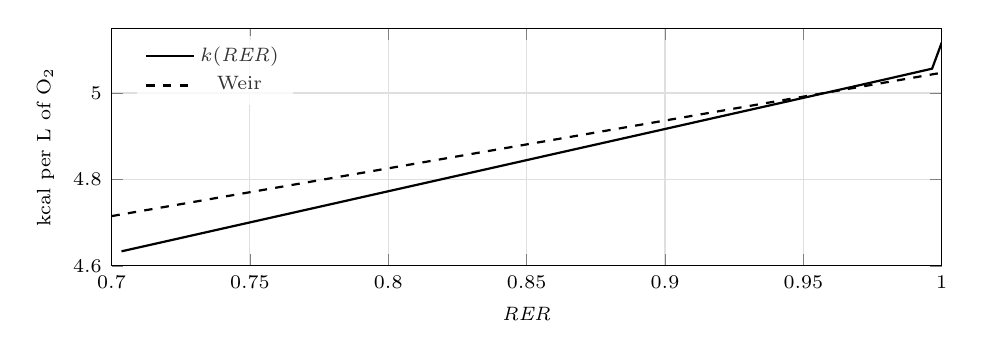
\begin{tikzpicture}
\begin{axis}[
  width=\linewidth, height=4.6cm,
  xmin=0.70, xmax=1.00, xlabel={\RER},
  ylabel={kcal per L of O$_2$}, ymin=4.6, ymax=5.15, grid=major, grid style={gray!25},
  xticklabel style={/pgf/number format/fixed,/pgf/number format/precision=2},
  yticklabel style={/pgf/number format/fixed,/pgf/number format/precision=1},
  tick label style={font=\scriptsize}, label style={font=\scriptsize},
  legend style={font=\scriptsize, at={(0.03,0.97)}, anchor=north west, draw=none, fill=white, fill opacity=0.8}]
\addplot[thick, black] coordinates {
 (0.7036,4.6337) (0.72,4.6573) (0.74,4.6862) (0.76,4.7150) (0.78,4.7438) (0.80,4.7727)
 (0.82,4.8015) (0.84,4.8303) (0.86,4.8592) (0.88,4.8880) (0.90,4.9168) (0.92,4.9457)
 (0.94,4.9745) (0.96,5.0033) (0.98,5.0322) (0.9965,5.0564) (1.00,5.1168)};
\addlegendentry{$k(\RER)$}
\addplot[thick, dashed, black] coordinates {(0.70,4.7152) (1.00,5.0470)};
\addlegendentry{Weir}
\end{axis}
\end{tikzpicture}
\end{minipage}

\medskip
\textbf{Result:} the difference is below 1.5\,\% over the whole range. The small jump at
the end of the curve, between $\RER=0.9965$ and $1.00$, is because in this segment fat is
already zero (section~\ref{sec:jw-rer}) and $k$ is no longer the straight line: only
$e_{\CHO}\cdot g_{\CHO}$ remains. That is why the 1.00 row gives $+1.4\,\%$.
\end{requadre}

\subsection{Oxygen uptake from energy}\label{sec:vo2-calcul}
Once $k$ is computed, we apply~\eqref{eq:vo2}. The units work out:
\[
  \VO(t)=\frac{E(t)}{k\bigl(\RER(t)\bigr)}\qquad
  \Bigl[\frac{\kcal/\mathrm{min}}{\kcal/\mathrm{L}}=\frac{\mathrm{L}}{\mathrm{min}}\Bigr].
\]
For example, if 12~kcal/min are expended and each litre releases 4.94, the oxygen uptake is
$12/4.94=2.43$~L/min. This value can be compared with $\VOmax$ to detect impossible values.

\subsection{Oxidation rate of each substrate}\label{sec:grams}
We go back to the equations of Jeukendrup and Wallis with the
\RER~\eqref{eq:jw-cho-rer}--\eqref{eq:jw-fat-rer}:
\[
  \cho(t)=\VO(t)\cdot\bigl(4.210\cdot\RER(t)-2.962\bigr).
\]
We insert the oxygen uptake we have obtained, $\VO(t)=E(t)/k\bigl(\RER(t)\bigr)$~\eqref{eq:vo2}:
\[
  \cho(t)=\frac{E(t)}{k\bigl(\RER(t)\bigr)}\cdot\bigl(4.210\cdot\RER(t)-2.962\bigr).
\]
And with the simple form of $k$~\eqref{eq:klin} we get a formula that depends only on the
energy and the \RER:
\begin{align}
  \cho(t) &= E(t)\cdot\frac{4.210\cdot\RER(t)-2.962}{3.620+1.442\cdot\RER(t)}, \label{eq:cho-final}\\[4pt]
  \fat(t) &= E(t)\cdot\frac{1.695-1.701\cdot\RER(t)}{3.620+1.442\cdot\RER(t)}. \label{eq:fat-final}
\end{align}

These formulas hold between $\RER\approx0.704$ and $0.9965$. Outside this range, the
extremes are set to zero (section~\ref{sec:jw-rer}) and~\eqref{eq:k} is used. The amount of
energy comes from Garmin, and the \RER\ determines how it is split.

\begin{requadre}{``Garmin energy conservation principle''}
\textbf{What is checked:} that the condition on which the method is built holds
(section~\ref{sec:objectiu}): the energy of the computed grams is exactly the energy given
by Garmin.

\smallskip
Multiplying each rate by its energy per gram and adding:
\begin{equation}
\begin{aligned}
  e_{\CHO}\cdot\cho(t)+e_{\FAT}\cdot\fat(t)
  &=\VO(t)\cdot\Bigl(e_{\CHO}\cdot g_{\CHO}\bigl(\RER(t)\bigr)+e_{\FAT}\cdot g_{\FAT}\bigl(\RER(t)\bigr)\Bigr)\\
  &=\frac{E(t)}{k\bigl(\RER(t)\bigr)}\cdot k\bigl(\RER(t)\bigr)=E(t) .
\end{aligned}
  \label{eq:conservacio}
\end{equation}
\textbf{Result:} it holds exactly, whatever the \RER, also at the extremes where one of the
two $g$ values is zero.

\smallskip
This happens because $k$ has been computed with the same numbers as the equations of
Jeukendrup and Wallis. It does not justify the values 4.1 and 9.3 (it would hold with any
pair of values, if $k$ is computed with the same ones), but it guarantees that the amount of
energy is always Garmin's, and that the method only splits it between the two substrates.
With a fixed $k$ or with Weir's, oxygen uptake would be practically the same, but the
energy of the grams would not match Garmin's (differences of up to 4\,\% and 1.5\,\%).
\end{requadre}

% =====================================================================
\section{Error as a function of the RER}\label{sec:sensibilitat}
% =====================================================================

The \RER\ is estimated from \FC, and each person's real value can be somewhat different
(section~\ref{sec:limitacions}). This section studies how the computed grams change when
the \RER\ varies by an amount $\varepsilon$, with the energy $E$ fixed (Garmin's). For
simplicity, we do not write the dependence on $t$.

Formulas~\eqref{eq:cho-final}--\eqref{eq:fat-final} have the form
\[
  \cho(\RER)=E\cdot\frac{a\cdot\RER-b}{k(\RER)},\qquad
  \fat(\RER)=E\cdot\frac{a'-b'\cdot\RER}{k(\RER)},\qquad
  k(\RER)=c+d\cdot\RER,
\]
with $a=4.210$, $b=2.962$, $a'=1.695$, $b'=1.701$, $c=3.620$ and $d=1.442$.

\paragraph{Exact variation.} If the \RER\ goes from $\RER$ to $\RER+\varepsilon$:
\begin{equation}
\begin{aligned}
  \Delta\cho&=\cho(\RER+\varepsilon)-\cho(\RER)
  =E\cdot\left(\frac{a\,(\RER+\varepsilon)-b}{k(\RER+\varepsilon)}-\frac{a\cdot\RER-b}{k(\RER)}\right)\\[4pt]
  &=\frac{(a\,c+b\,d)\cdot E\cdot\varepsilon}{k(\RER)\cdot k(\RER+\varepsilon)}
  =\frac{19.51\cdot E\cdot\varepsilon}{k(\RER)\cdot k(\RER+\varepsilon)} ,
\end{aligned}
\label{eq:dcho}
\end{equation}
and, in the same way,
\begin{equation}
  \Delta\fat=-\frac{(b'c+a'd)\cdot E\cdot\varepsilon}{k(\RER)\cdot k(\RER+\varepsilon)}
  =-\frac{8.60\cdot E\cdot\varepsilon}{k(\RER)\cdot k(\RER+\varepsilon)} .
\label{eq:dfat}
\end{equation}
In the numerator, the terms with \RER\ cancel out. The variation is proportional to
$\varepsilon$ and to the energy $E$, and the \RER\ only appears through $k$, which varies
little.

The total energy does not change: $4.1\cdot19.51\approx9.3\cdot8.60\approx80$, so the
energy gained by carbohydrate is the energy lost by fat. This is the ``Garmin energy
conservation principle''~\eqref{eq:conservacio}.

\paragraph{Approximation.} For small variations, $k(\RER+\varepsilon)\approx k(\RER)$:
\[
  \Delta\cho\approx\frac{19.51}{k(\RER)^2}\cdot E\cdot\varepsilon,\qquad
  \Delta\fat\approx-\frac{8.60}{k(\RER)^2}\cdot E\cdot\varepsilon .
\]
The error of this step is very small: less than 1.5\,\% even with $\varepsilon=0.05$.

\paragraph{Bounds.} Within the valid range of the \RER\ (0.704--0.9965), $k$ goes from 4.63
to 5.06 (table~\ref{tab:sens}).

\begin{table}[H]
\centering
\caption{Approximate factors of~\eqref{eq:dcho}--\eqref{eq:dfat}, at the ends and in the
middle of the valid \RER\ range.}
\label{tab:sens}
\small
\begin{tabular}{@{}ccccc@{}}
\toprule
\RER & $k$ (kcal/L) & $k^2$ & $\dfrac{19.51}{k^2}$ & $\dfrac{8.60}{k^2}$ \\[6pt]
\midrule
0.704  & 4.63 & 21.5 & 0.91 & 0.40 \\
0.85   & 4.85 & 23.5 & 0.83 & 0.37 \\
0.9965 & 5.06 & 25.6 & 0.76 & 0.34 \\
\bottomrule
\end{tabular}
\end{table}

\noindent The carbohydrate factor always lies between 0.76 and 0.91. Taking the middle
value, 0.83, the error is at most $\pm9$\,\%. With $E$ in kcal/min, and multiplying by 60
to convert to g/h:
\begin{equation}
  \Delta\cho\approx0.83\cdot E\cdot\varepsilon~[\mathrm{g/min}]
  \approx50\cdot E\cdot\varepsilon~[\mathrm{g/h}],\qquad
  \Delta\fat\approx-0.37\cdot E\cdot\varepsilon~[\mathrm{g/min}]
  \approx-22\cdot E\cdot\varepsilon~[\mathrm{g/h}].
\label{eq:dsimple}
\end{equation}

\paragraph{Example.} With $E=12$~kcal/min and $\varepsilon=0.01$:
$\Delta\cho\approx50\cdot12\cdot0.01=6$~g/h and $\Delta\fat\approx-22\cdot12\cdot0.01
\approx-2.6$~g/h. With the exact formula~\eqref{eq:dcho} we get 5.9~g/h with $\RER=0.86$
and 5.6~g/h with $\RER=0.95$. If a person's real \RER\ differs by 0.04 from the estimate,
the difference is about 24~g/h of carbohydrate.

\begin{conclusio}
\begin{itemize}[leftmargin=*]
  \item The variation of the grams is proportional to the variation of the \RER\ and to the
        energy, and it hardly depends on the value of the \RER.
  \item \textbf{Rule of thumb: $\Delta\cho\approx50\cdot E\cdot\varepsilon$~g/h and
        $\Delta\fat\approx-22\cdot E\cdot\varepsilon$~g/h} ($E$ in kcal/min). At
        12~kcal/min, each 0.01 of \RER\ is about 6~g/h of carbohydrate, and about 2.6~g/h of
        fat in the opposite direction.
  \item The total energy does not change: the \RER\ only determines how it is split.
  \item That is why what matters most is to have the thresholds, especially $LT_2$, set
        correctly.
\end{itemize}
\end{conclusio}

% =====================================================================
\section{Computing \texorpdfstring{$\mathit{CHO}_{\mathrm{total}}$ and $\mathit{FAT}_{\mathrm{total}}$}{CHO total and FAT total}}\label{sec:total}
% =====================================================================

The aim~\eqref{eq:totals} asks for the cumulative total, that is, the integral of the rates
over the activity. This section explains how it is computed with the data Garmin gives.

\subsection{Garmin gives the cumulative energy}
Garmin does not give the rate $E(t)$, but the cumulative energy $E_{\tot}(t)$~\eqref{eq:etotal},
as an integer number of kilocalories that goes up one by one \citep{garminciq}. In real
activities with a Garmin watch it has been checked that:
\begin{itemize}
  \item the counter is the \emph{total} energy (resting included): its final value matches
        the activity total;
  \item it goes up by 1~kcal each time, at intervals that depend on intensity (every
        5--7~s when running);
  \item it does not advance while the timer is stopped.
\end{itemize}
It can be read, together with \FC, about once per second.

\subsection{Intervals between increments}
Each time the counter goes up, it closes an interval $j$, between instants $t_{j-1}$ and
$t_j$, with an energy
\begin{equation}
  \Delta E_j=E_{\tot}(t_j)-E_{\tot}(t_{j-1})=\int_{t_{j-1}}^{t_j}E(t)\,dt .
  \label{eq:deltaE}
\end{equation}
It is the integral of the energy over that interval, and we do not have to compute it: the
Garmin counter gives it. It is normally 1~kcal.

\paragraph{The grams of each interval.} They are the integral of the
rate~\eqref{eq:cho-final} over that interval:
\[
  \Delta\cho_j=\int_{t_{j-1}}^{t_j}\cho(t)\,dt
  =\int_{t_{j-1}}^{t_j}E(t)\cdot\frac{g_{\CHO}\bigl(\RER(t)\bigr)}{k\bigl(\RER(t)\bigr)}\,dt .
\]
The interval lasts about 5~s, and we take the \RER\ as constant over it, equal to the mean
of the per-second \RER\ values (figure~\ref{fig:comptador}):
\[
  \RERi_j=\frac{\sum_i\RER_i\cdot\Delta t_i}{\sum_i\Delta t_i} .
\]
Then $g_{\CHO}/k$ is a fixed number and comes out of the integral. The remaining integral
is that of the energy, which is $\Delta E_j$~\eqref{eq:deltaE}:
\begin{align}
  \Delta\cho_j &\approx\frac{g_{\CHO}(\RERi_j)}{k(\RERi_j)}\cdot\int_{t_{j-1}}^{t_j}E(t)\,dt
  =\Delta E_j\cdot\frac{g_{\CHO}(\RERi_j)}{k(\RERi_j)}, \label{eq:interval}\\
  \Delta\fat_j &\approx\Delta E_j\cdot\frac{g_{\FAT}(\RERi_j)}{k(\RERi_j)} . \notag
\end{align}
The only approximation is taking the \RER\ as constant for a few seconds. Since the
intervals are so short, it hardly changes the result.

\begin{figure}[H]
\centering
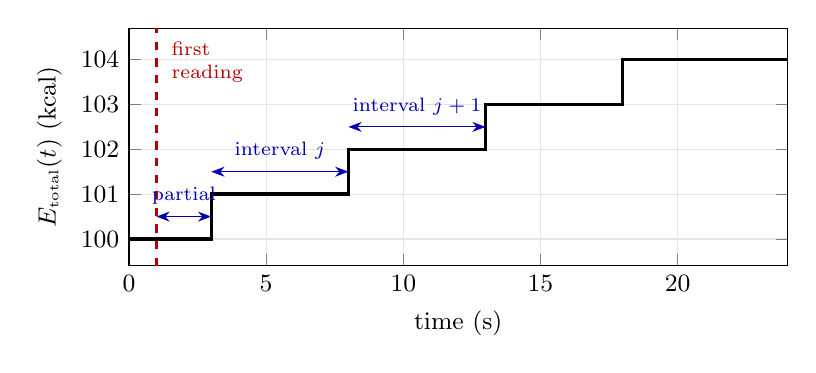
\begin{tikzpicture}
\begin{axis}[
  width=0.82\textwidth, height=4.6cm,
  xmin=0, xmax=24, ymin=99.4, ymax=104.7,
  xlabel={time (s)}, ylabel={$E_{\tot}(t)$ (kcal)},
  ytick={100,101,102,103,104},
  tick label style={font=\small}, label style={font=\small},
  grid=major, grid style={gray!20}]
\addplot[const plot, very thick, black] coordinates {
 (0,100) (3,101) (8,102) (13,103) (18,104) (24,104)};
\draw[dashed, red!70!black, thick] (axis cs:1,99.4) -- (axis cs:1,104.7);
\node[font=\scriptsize, red!70!black, anchor=north west, align=left] at (axis cs:1.2,104.6) {first\\reading};
\draw[{Stealth}-{Stealth}, blue!70!black] (axis cs:1,100.5) -- (axis cs:3,100.5);
\node[font=\scriptsize, blue!70!black, anchor=south] at (axis cs:2,100.55) {partial};
\draw[{Stealth}-{Stealth}, blue!70!black] (axis cs:3,101.5) -- (axis cs:8,101.5);
\node[font=\scriptsize, blue!70!black, anchor=south] at (axis cs:5.5,101.55) {interval $j$};
\draw[{Stealth}-{Stealth}, blue!70!black] (axis cs:8,102.5) -- (axis cs:13,102.5);
\node[font=\scriptsize, blue!70!black, anchor=south] at (axis cs:10.5,102.55) {interval $j+1$};
\end{axis}
\end{tikzpicture}
\caption{Garmin's cumulative energy counter. Each 1~kcal increment closes an interval,
whose energy is split with~\eqref{eq:interval} and the mean \RER\ of the interval. The first
reading falls at any point between two increments, so the first interval is partial.}
\label{fig:comptador}
\end{figure}

\subsection{Totals}
The totals~\eqref{eq:totals} are the integral over the whole activity, which is the sum of
the integrals over each interval:
\begin{equation}
  \cho_{\tot}(T)=\int_0^T\cho(t)\,dt=\sum_j\int_{t_{j-1}}^{t_j}\cho(t)\,dt=\sum_j\Delta\cho_j ,
\end{equation}
and likewise for fat. Garmin does the integral of the energy for us; we only need to add up
the pieces. By the ``Garmin energy conservation principle''~\eqref{eq:conservacio}, applied
to each interval,
\begin{equation}
  e_{\CHO}\cdot\cho_{\tot}(T)+e_{\FAT}\cdot\fat_{\tot}(T)=E_{\tot}(T)-E_{\tot}(t_0):
\end{equation}
the energy that is split is exactly the energy Garmin has counted since the first reading
$t_0$, with no summation error. If the counter is not read for a while, no energy is lost:
the next increment already includes it. The energy the counter already held at the first
reading is not split. Nothing accumulates while the timer is stopped.

% =====================================================================
\section{Example}\label{sec:exemple}
% =====================================================================

An athlete with $LT_2=166$~bpm and $\FCmax=180$~bpm runs at 150~bpm, and from the Garmin
counter the expenditure rate is $E=12$~kcal/min.
\begin{enumerate}
  \item \textbf{\RER}~\eqref{eq:rer}: $LT_1=0.89\cdot166=147.7$~bpm, so
        \[
          \RER=0.91+\frac{150-147.7}{166-147.7}\cdot(0.98-0.91)=0.919 .
        \]
  \item \textbf{Grams per litre}~\eqref{eq:gc}--\eqref{eq:gf}:
        $g_{\CHO}=4.210\cdot0.919-2.962=0.906$~g/L and
        $g_{\FAT}=1.695-1.701\cdot0.919=0.132$~g/L.
  \item \textbf{Energy per gram}~\eqref{eq:e}: $e_{\CHO}=4.1$ and $e_{\FAT}=9.3$~kcal/g.
  \item \textbf{Energy per litre}~\eqref{eq:k}:
        $k=4.1\cdot0.906+9.3\cdot0.132=4.944$~kcal/L.
  \item \textbf{Oxygen uptake}~\eqref{eq:vo2}: $\VO=12/4.944=2.43$~L/min.
  \item \textbf{Oxidation rate}: $\cho=2.43\cdot0.906=2.20$~g/min
        and $\fat=2.43\cdot0.132=0.32$~g/min, that is, 132~g/h of carbohydrate and
        19~g/h of fat.
\end{enumerate}
Starting condition~\eqref{eq:conservacio}: $4.1\cdot2.198+9.3\cdot0.321=12.00$~kcal/min.

% =====================================================================
\section{Sources of error and limitations}\label{sec:limitacions}
% =====================================================================

Table~\ref{tab:errors} lists the sources of error, classified by whether they affect the
amount of energy or its split.

\begin{table}[H]
\centering
\caption{Sources of error of the method.}
\label{tab:errors}
\small
\begin{tabularx}{\textwidth}{@{}>{\raggedright\arraybackslash}p{3.6cm} L >{\raggedright\arraybackslash}p{2.4cm}@{}}
\toprule
Source & Description & Affects \\
\midrule
Garmin's energy & Manufacturer's computation, with known errors in wearable devices
\citep{shcherbina2017,fuller2020}; it depends on the user profile (body mass, age,
maximum \FC, $\VOmax$). & Amount (and grams, in the same proportion) \\
Estimated \RER & Typical population values; each person can differ by about $\pm0.04$
\citep{goedecke2000}; it depends on the thresholds, especially $LT_2$. & Split \\
Exercise duration & The real \RER\ decreases as exercise goes on
\citep{rothschild2022}; the model does not account for it. & Split (CHO overestimated
from the second hour on) \\
Diet, fasting, fitness & Fasting or a low-carbohydrate diet lower the \RER; see
\citep{chofatfc2026}. & Split \\
Protein & The equations ignore protein oxidation \citep{frayn1983,jeukendrup2005}: its
energy, which is small, is assigned to carbohydrate and fat. & Split (small) \\
Anaerobic glycolysis & Above $LT_2$ glycogen is used that does not appear in the oxidation
computed from gases. & Split (CHO underestimated) \\
\bottomrule
\end{tabularx}
\end{table}

The split cannot be adjusted with any Garmin data, because Garmin says nothing about
carbohydrate and fat. Validating it requires an exercise test with a gas analyser. The
energy, on the other hand, is as good as Garmin's estimate: if that improves, the result
improves without changing anything.

% =====================================================================
\section{Real-time estimate of mean CHO use}\label{sec:implementacio}
% =====================================================================

\paragraph{What we want.} A real-time estimate of how many grams of carbohydrate per hour
are being oxidised, giving more weight to the last minutes.

\paragraph{The problem.} The grams arrive in jumps. At each 1~kcal increment (every 5~s or
so) the grams of the interval~\eqref{eq:interval} come in all at once, and between
increments none come in. The per-second rate is either zero or a spike, and it is useless as
an estimate.

\paragraph{First idea: the mean over the whole activity.} Divide the total grams by the
time. It is stable, but after an hour it hardly moves when intensity changes. It makes sense
as a summary at the end of the activity.

\paragraph{The solution: a mean that weighs the last minutes more.} An exponential moving
average is used \citep{hunter1986}. In words: at each reading (once per second), the
previous value loses a small part of its weight, $\Delta t/\tau$, and the new grams divided
by $\tau$ come in. With $\tau=15$~min:
\begin{equation}
  \bar r_i=\Bigl(1-\frac{\Delta t_i}{\tau}\Bigr)\cdot\bar r_{i-1}+\frac{\Delta\cho_i}{\tau},
  \label{eq:ema}
\end{equation}
where $\bar r_i$ is the estimate, in g/min (multiplied by 60, in g/h); $\Delta t_i$ is the
time since the previous reading, and $\Delta\cho_i$ the grams assigned at this reading
(zero if there has been no increment).

\paragraph{What $\tau=15$~min means.} The estimate is, roughly, the use over the
\textbf{last 15 minutes}, with the most recent part weighing more. It is like the
``memory'' of the average: what happened 15 minutes ago still counts a little, 30 minutes
ago very little, and 45 minutes ago it is practically forgotten. For example, when going
from an easy pace to a hard one, the estimate does not jump at once: after 15 minutes it has
made about 2/3 of the change, and after 45 minutes almost all of it.

\paragraph{Why 15 minutes.} With a shorter time the estimate reacts faster, but it jumps
around more; with a longer time it is more stable, but it lags behind. 15 minutes is a
compromise, and it is roughly the time scale on which decisions about when to eat are made.

\paragraph{Start.} The first interval is partial (figure~\ref{fig:comptador}), but it
carries a whole kilocalorie, so its rate can be several times higher than the real one. If
the average started with this value, the error would take a long time to disappear. That is
why, during the first minute, the real mean (grams divided by time) is used, where this
error is already spread over a dozen intervals, and from then on the moving average starts
from this value.

% =====================================================================
\section{Conclusions}
% =====================================================================

The starting point of this work is a condition: the energy of the computed grams must be
the energy given by Garmin, which uses more information than \FC\ alone. The method does
not recompute the energy; it only splits it between carbohydrate and fat.

The equations of Jeukendrup and Wallis compute the oxidation rate of carbohydrate and fat
from oxygen uptake and the \RER. Without a gas analyser, the \RER\ can be estimated from
\FC, and oxygen uptake from the energy given by Garmin: it is enough to divide it by the
energy released per litre of oxygen, $k(\RER)$. This key piece is computed with the same
equations and with the energy per gram of carbohydrate (4.1~kcal) and fat (9.3~kcal),
values that agree with the literature and with classical calorimetry. Since $k$ varies
little, oxygen uptake comes almost only from the energy. And since it is computed with the
same numbers, the energy of the resulting grams is exactly Garmin's, both at each instant
and in the total. In the end there are two well-separated sources of error: the amount of
energy, which comes from Garmin, and the split between carbohydrate and fat, which depends
on the estimated \RER\ and, above all, on whether the thresholds are set correctly.

The method would work with any device that gives the total energy of the activity, but the
checks on how the energy counter behaves have been made with Garmin.

% =====================================================================
\begin{thebibliography}{99}
\small

\bibitem[Atwater and Bryant(1900)]{atwater1900}
Atwater WO, Bryant AP.
\newblock The availability and fuel value of food materials.
\newblock \emph{Storrs Agricultural Experiment Station 12th Annual Report}. 1900:73--110.

\bibitem[CHO/FAT Metabolic Pro project(2026)]{chofatfc2026}
CHO/FAT Metabolic Pro project.
\newblock Estimating carbohydrate and fat oxidation from heart rate. 2026.
\newblock \webprojecte

\bibitem[Firstbeat Technologies(2007)]{firstbeat2007}
Firstbeat Technologies Ltd.
\newblock An energy expenditure estimation method based on heart rate measurement.
\newblock White paper. Jyväskylä: Firstbeat Technologies; 2007.

\bibitem[Frayn(1983)]{frayn1983}
Frayn KN.
\newblock Calculation of substrate oxidation rates in vivo from gaseous exchange.
\newblock \emph{J Appl Physiol}. 1983;55(2):628--634.

\bibitem[Fuller et~al.(2020)]{fuller2020}
Fuller D, Colwell E, Low J, et~al.
\newblock Reliability and validity of commercially available wearable devices for
  measuring steps, energy expenditure, and heart rate: systematic review.
\newblock \emph{JMIR Mhealth Uhealth}. 2020;8(9):e18694.

\bibitem[Garmin(2026)]{garminciq}
Garmin Ltd.
\newblock Connect IQ SDK 9.2.0, API documentation: \texttt{Toybox.Activity.Info}.
  2026.

\bibitem[Goedecke et~al.(2000)]{goedecke2000}
Goedecke JH, St~Clair Gibson A, Grobler L, Collins M, Noakes TD, Lambert EV.
\newblock Determinants of the variability in respiratory exchange ratio at rest and during
  exercise in trained athletes.
\newblock \emph{Am J Physiol Endocrinol Metab}. 2000;279(6):E1325--E1334.

\bibitem[Hunter(1986)]{hunter1986}
Hunter JS.
\newblock The exponentially weighted moving average.
\newblock \emph{J Qual Technol}. 1986;18(4):203--210.

\bibitem[Jeukendrup(2014)]{jeukendrup2014}
Jeukendrup AE.
\newblock A step towards personalized sports nutrition: carbohydrate intake during
  exercise.
\newblock \emph{Sports Med}. 2014;44(Suppl 1):S25--S33.

\bibitem[Jeukendrup and Wallis(2005)]{jeukendrup2005}
Jeukendrup AE, Wallis GA.
\newblock Measurement of substrate oxidation during exercise by means of gas
  exchange measurements.
\newblock \emph{Int J Sports Med}. 2005;26(Suppl 1):S28--S37.

\bibitem[Livesey and Elia(1988)]{livesey1988}
Livesey G, Elia M.
\newblock Estimation of energy expenditure, net carbohydrate utilization, and net fat
  oxidation and synthesis by indirect calorimetry: evaluation of errors with special
  reference to the detailed composition of fuels.
\newblock \emph{Am J Clin Nutr}. 1988;47(4):608--628.

\bibitem[Péronnet and Massicotte(1991)]{peronnet1991}
Péronnet F, Massicotte D.
\newblock Table of nonprotein respiratory quotient: an update.
\newblock \emph{Can J Sport Sci}. 1991;16(1):23--29.

\bibitem[Rothschild et~al.(2022)]{rothschild2022}
Rothschild JA, Kilding AE, Stewart T, Plews DJ.
\newblock Factors influencing substrate oxidation during submaximal cycling: a modelling
  analysis.
\newblock \emph{Sports Med}. 2022;52(11):2775--2795.

\bibitem[Shcherbina et~al.(2017)]{shcherbina2017}
Shcherbina A, Mattsson CM, Waggott D, et~al.
\newblock Accuracy in wrist-worn, sensor-based measurements of heart rate and energy
  expenditure in a diverse cohort.
\newblock \emph{J Pers Med}. 2017;7(2):3.

\bibitem[Swain and Leutholtz(1997)]{swain1997}
Swain DP, Leutholtz BC.
\newblock Heart rate reserve is equivalent to \%VO$_2$ reserve, not to
  \%VO$_2$max.
\newblock \emph{Med Sci Sports Exerc}. 1997;29(3):410--414.

\bibitem[Weir(1949)]{weir1949}
Weir JB de V.
\newblock New methods for calculating metabolic rate with special reference to
  protein metabolism.
\newblock \emph{J Physiol}. 1949;109(1--2):1--9.

\end{thebibliography}

\end{document}
